% THIS IS SIGPROC-SP.TEX - VERSION 3.1
\documentclass{llncs}

% Additional packages
\usepackage{graphicx}
\usepackage{color}
\usepackage{url}
\usepackage{algorithm}
\usepackage[noend]{algpseudocode}
\usepackage{amsmath}
%\usepackage{amsthm}
\usepackage{amsfonts}
\usepackage{amssymb}
\usepackage{booktabs}
\usepackage{multirow}
\usepackage{ifpdf}
% Custom commands
\usepackage{custom_commands}

%\newcommand{\prg}[1]{\paragraph{#1}}
\newcommand{\prg}[1]{\textbf{#1}.}

\renewcommand{\note}[1]{{\color{red}{#1}\par}}

\newcommand{\Siren}{\textsc{Siren}}
\newcommand{\ReReMi}{\textsc{ReReMi}}

\def\verExample{1}
\def\verE{0}

\begin{document}


\title{Siren: An Interactive Tool for Mining and Visualizing Geospatial Redescriptions}

%\numberofauthors{2} 
\author{
Esther Galbrun\inst{1}
\and
Pauli Miettinen\inst{2}
}

\institute{
  Helsinki Institute for Information Technology,\\
  Department of Computer Science, \\
  University of Helsinki, Finland,\\
  \email{galbrun@cs.helsinki.fi}
\and
  Max Planck Institute for Informatics, \\
  Saarbr{\"u}cken, Germany,\\
  \email{pmiettin@mpi-inf.mpg.de}
}
 
\maketitle
\begin{abstract}
  \note{being re-written} 
  We discuss the importance of visualization and
  interactivity for data analysis throught the example of geospatial redescription mining.

  % Redescription mining is a powerful data analysis tool that aims at
  % finding alternative descriptions of the same entities.  In
  % particular, we consider geospatial redescription mining, that is,
  % the case where the entities are linked to geographical locations.  For
  % example, in biology, an important task is to identify the
  % bioclimatic constraints that allow some species to survive, that is,
  % to describe geographical regions in terms of both the fauna that
  % inhabits them and their bioclimatic conditions.

  We argue that interactivity of the mining tool and intuitive
  visualization of the results are key elements towards a successful
  analysis, but that there exist dangers to the extensive use of user
  interaction in data mining.
\end{abstract}

\section{Introduction}
\note{TODO: start visual and interactive data mining more generally?}

Finding multiple ways to characterize the same entities is a problem
that appears in many areas of science.  In medical sciences, one might
want to find a subset of patients sharing similar symptoms and similar
genes. Describing geographical regions in terms of both their
bioclimatic conditions and the fauna that inhabits them is another
example.  A simple example of a redescription in this setting could
state that areas where Moose live are areas where February's maximum
temperature is between $-10$ and $0$ degrees Celsius and July's
maximum temperature between $12$ and $25$ degrees Celsius.
%This is actually the redescription shown in the foreground panel of
%Figure~\ref{fig:both_panels}.

The results of redescription mining, the redescriptions, can be
approached from two points of view. On one hand, by considering the
variables and conditions appearing in the queries, which provide
valuable information in themselves; on the other hand, by studying the
support set of the redescriptions, i.e.\ the subset of entities where
both queries of a redescription hold. 
 
\note{I don't think we can have a strict division between visualizing results and
  interacting with the mining algorithm... It could be partly using
  visual means to interact with the mining process (select areas,
  scatter plot with sliders)}

To analyse the
redescriptions, the ability to visualize the support sets is very
helpful. With geospatial data, the visualization is rather simple:
plot the support sets in a map. But just plotting the results on a map
is not enough: the user must also be able to interact with the
program. This interaction can be conceptually divided in two
sub-phases: interacting with the data mining algorithm and interacting
with the result visualization. A third level of interaction happens
between these two conceptual phases: the user moves back-and-forth
between issuing commands to find new results and examining the
already-found results. We argue that a good interactive data mining
tool should facilitate all three types of interaction. In this paper
we discuss about ways to facilitate this interaction in the process of
mining redescriptions. We then present a pair of algorithms, \ReReMi\
and \Siren, and explain how they implement interactivity and
visualization for redescription mining. Lastly, we discuss some
possible pitfalls associated with interactive, visual redescription
mining. But first, we formally define the redescription mining
problem.

\section{Redescription Mining}
\label{sec:redescription-mining}

Redescription mining aims at simultaneously finding multiple
descriptions of a subset of entities which is not previously
specified.  This is in contrast with other methods like Emerging
Patterns Mining (EPM), Contrast Set Mining (CSM) and Subgroup
Discovery (SD) (see \cite{kralj09supervised} for a unifying survey) or
general classification methods, where target subsets of entities are
specified via labels.  Currently, redescription mining is a purely
descriptive approach, its predictive power remains to be explored.
Since its introduction in~\cite{ramakrishnan04turning} various
algorithms have been proposed for Boolean redescription mining, based
on approaches including decision
trees~\cite{ramakrishnan04turning,kumar07redescription},
co-clusters~\cite{parida05redescription}, and frequent
itemsets~\cite{gallo08finding}. In~\cite{galbrun11black}, we extended
redescription mining to categorical and numerical variables.

More formally, we consider data that contains entities with two sets
of characterizing variables, e.g.\ the fauna and the bioclimatic
conditions. 
Boolean variables can be interpreted as a truth value
assignment in a natural way.  For categorical and real-valued
variables, truth value assignments are induced by relations $[v=c]$
and $[a \leq v \leq b]$, respectively, where $c$ is some category and
$[a, b]$ an interval.  These truth assignments and their negations
constitute \emph{literals} which can be combined using the Boolean
operators $\land$ (and) and $\lor$ (or) to form \emph{queries}.
We refer to the two sets of variables informally as left and right
hand side data, and the queries over them, respectively, as left and
right hand side queries.
Then, a redescription is simply a pair of queries over variables from the
two sets.  The support of a query is the subset of entities for which
the query holds true.  The \emph{accuracy} of a redescription is
measured by the \emph{Jaccard coefficient} of the supports of its two
queries.
The task consists in finding accurate redescriptions, in other words, pairs of
queries, one query for both sets of variables, such that both queries
describe almost the same set of entities.

When the data is geospatial, that is, the entities are connected to
geographical locations, the latter approach becomes even more
important. A meaningful geospatial redescription should define
coherent areas using expressive queries.

Niche-finding is a particular instance of geospatial redescription
mining ---and a task of great importance for biologists.  The
bioclimatic constraints that must be met for a certain species to
survive constitute that species' bioclimatic envelope, or
niche~\cite{grinnell17niche}.  Finding such envelopes can help, e.g.\
to predict the results of global warming~\cite{pearson03predicting}.
A number of methods, involving regression, neural networks, and
genetic algorithms (see~\cite{soberon05interpretation}) have been
developed over the past ten year to model the bioclimatic envelope,
\textsc{BIOMOD}~\cite{thuiller09biomod} being a good example of a
modelling tool used in this domain.  But to the best of our knowledge,
none of these methods allows automatically finding both the set of
species and their envelope.

\section{Goals for Interactive and Visual Redescription Mining}
\label{sec:goals-inter-visu}

In this section we discuss on our goals for an interactive and visual
redescription mining tool. Some of these goals are general to any
interactive and visual data mining tool (and we spend less time on
discussing why they are desirable), some specific for the
redescription mining. We divide the discussion between interaction and
visualization, though we emphasize that these goals are not independent.

\subsection{Goals for Visualization}
\label{sec:goals-visualization}
As a basis for our discussion, we use the taxonomy of interations for
visual analytics proposed by Heer and
Shneiderman~\cite{Heer:2012:IDV:2133806.2133821}. The bold-face terms
correspond to their taxonomy.

\paragraph{Data and View Specification.}
The most fundamental goal when designing a tool for visual data
analysis is, of course, to have a good \textbf{visualization}. With
geospatial redescriptions, a map is the most natural option. Thus our
tool should be able to plot the redescriptions on a map. But besides a
visualization, the user needs means to \textbf{filter} and
\textbf{sort} the results mined. In the case of redescription mining,
the user should be able to sort the redescriptions based on different
criteria, such as the accuracy of the redescription, the size of its
support, its $p$-value, or the length of the queries (i.e.\ their
number of literals).  The user should be able to \textbf{filter} the
redescriptions based on these same criteria as well as on, e.g. the
described geographical area.  To some extent, filtering can be
regarded as sorting with a cut-off value. Hence, sorting and filtering
should naturally use the same criteria and similar result display.
During the analysis, the user should be allowed to \textbf{derive} new
data. That is introducing new variables as aggregate of the existing
ones or modifying the split between variables while mining
redescriptions.

\paragraph{View Manipulation.}
In order to manipulate the views, the user needs to be able to
\textbf{select} the data he wants to visualize. In the present case,
he can primarily choose a redescription to plot. Then, he can edit the
queries, modifying literals and altering the bounds of real valued
variables. In addition, it can be useful to obtain information about
the state of the variables and what makes a query hold or not in a
particular location by clicking or hovering over a dot in the map.
The user might need to \textbf{navigate} inside the view, typically
looking first at the redescription over the whole area, before zooming
and panning to see more details. Several views and the data might need
to be \textbf{coordinated}.  Modifications made to a redescription
should be reflected immediately on the map(s). In addition, it could
be useful to allow the user to bind maps together, so that panning and
zooming are applied to all maps simultaneouly. In that way, detailed
comparison of the support of different redescription would be
facilitated.  Maps can be opened in detachable tabs, to be inspected
side by side or sequentially and be \textbf{organized} using the
system's windows tiling, or a dedicated one.

\paragraph{Process and Provenance.}
Undo and redo are minimal functionalities to allow reverting actions,
making interation safe and comfortable.  The user should be able to
save the current status of the analysis process, i.e. all current
redescriptions, opened lists and maps to punctuate the
process. \textbf{Recording} the interaction history and turning it
into editable and parameterizable macros provides a mean to repeat a
sequence of actions and automate repetitive tasks.  The tool should
support \textbf{annotation} in order to keep track of the thought path
during the analysis.  For example, this could be achieved by
generating annotable screen shots of the current window of interest,
and by adding comments to the interaction history and macros.
Organizing the history and macros into blocks would help clarifying
the logical structure of the analysis.  Furthermore, with the ability
to link to objects in the current environment such as redescriptions,
groups of entities or literals, they could be explicitely related to
each other.  Data analysis is often a collaborative effort, involving
several users. Then, \textbf{sharing} information becomes crucial.
Easy export and import of redescriptions lists, maps and macros,
possibly with comments and annotations is a very important feature
towards that aim.  Finally, giving clear names to the actions and
providing feedback on their application helps \textbf{guiding} users
along the analysis process. Example macros with detailed explanations,
to be replayed step-by-step, represent a good mean to introduce new
users to the tool.

\subsection{Goals for Interaction}
\label{sec:goals-interaction}
\note{Should we use interactivity here, as a general succession of interactions?}
\note{just some buzzwords now}

Any-time

Instat editing of redescriptions

When editing a real-valued literal,
showing a scatter plot of the entities based on the values of the
variable with colors indicating the current status of the rest of the
query can help the user fix the bounds, using sliders for
example.

Automated extension

Exclusion of variables/geographical areas

Pushing filtering into the mining process

$\ldots$


\section{The Algorithms}
\label{sec:algorithms}
\note{All explanations about the workings of ReReMi \& Siren here}

\Siren\ is an interactive tool for mining and visualizing geospatial
redescriptions. At its core is the \ReReMi\ redescription mining
algorithm~\cite{galbrun11black,galbrun12black}. This greedy algorithm
uses an efficient on-the-fly discretization technique to extend
redescription mining to categorical and numerical variables.

The search space of all Boolean formulae is too huge to be manageable.
Therefore, we need to restrict ourselves to a subset of formulae that
provides a good compromise between expressive power, difficulty of the
search, and interpretability.
For this purpose, we consider queries that can be parsed in linear
order, without trees, and allow every variable to appear only once.

Yet, the search space remains exponential and we still resort to a
heuristic pruning during the search.  We use a strategy similar to
beam-search to explore the solution space.  The basic idea is to
construct queries bottom-up, starting from singleton redescriptions
(i.e.\ both queries contain only one literal) and progressively
extending them by appending operators and
literals. % For example, we could start with a pair $(a,
% \lnot b)$, and try to extend it to $(a\land c, \lnot b)$, $(a \lor c,
% \lnot b)$, $(a \land \lnot c, \lnot b)$, etc.
After evaluating all
possible one-step extensions, we select the best candidates and extend
them in turn. This process stops when no new redescription can
be generated.

We exploit some
simple observations to make the computation of accuracy more
efficient. This allows to evaluate candidates faster, which is particularly important for an interactive tool.
We compute a \pValue{} that represents the probability that two random
queries with marginal probabilities (i.e.\ the fraction of entities
supporting them) equal to those of $q_\iLHS$ and $q_\iRHS$ have an
intersection equal to or larger than $\abs{\supp(q_\iLHS,
  q_\iRHS)}$. This probability uses the binomial distribution. The higher the
\pValue, the more likely it is to observe such a support for
independent queries, and the less significant the query. Redescriptions with too high \pValue{} can be filtered out.

Threading is employed to run mining tasks in the background. This preserves the tool's
interactivity while mainting the communication to provide feedback
about the ongoing mining.

\note{This had been commented out... We need to say these things don't we?}
\Siren\ and \ReReMi\ are implemented in Python.  The interface is
built with the \texttt{wxPython} Open Source GUI toolkit, ensuring
cross-platform compatibility. 
 The \texttt{matplotlib} library enables
to generate high quality figures, seamlessly integrated in the
interface.  \Siren\ allows for simple editing of the redescriptions
thanks to flexible parsing of different representations. It can handle
any data provided in a compatible format.  

\section{How the Algorithms Meet the Goals}
\label{sec:scenarios}

\note{The old use-case scenario text is a good basis for this, but
  needs to be re-worked a lot.\\
Do we want to talk only about the functionalities that are already implemented, can be reasonably implemented in a short delay, or any wishable functionality? And insert links to the goal section... 
}

We exemplify the usage of \Siren\ by going through a generic work-flow of
mining geospatial redescriptions, detailing typical steps in the process.  

This specific example concerns the application of \Siren\ on the task of bioclimatic niche finding using data
that describes spatial areas of Europe, squares of side roughly 50
kilometers.  The left hand side data contains information about the
mammals that live in these areas, while the right hand side consists
of bioclimatic variables\footnote{The data comes from two publicly available
datasets: European mammal atlas~\cite{mitchell-jones99atlas} and
Worldclim climate data~\cite{hijmans05very}.}.
Nonetheless, \Siren\ is a flexible tool that can be used with
different datasets from various application domains.

% A screenshot of the system,
% displaying a list of redescriptions with one
% particular redescription plotted on a map is shown in
% Figure~\ref{fig:both_panels}.

\prg{Initial redescription mining} A natural starting point for the
analysis of any given data is to use a redescription mining algorithm
to find an initial set of redescriptions.  This can be done withing
\Siren{} by running the extension mechanism on an empty redescription.

Following the principle of first providing an overview of the
results then focusing on specific items.
The redescriptions found are presented as a list, which extends as the
mining process progresses and supports sorting on various criteria.
Then, the user can select a redescription of his choice and visualize
it on a map.

\prg{Extending a redescription} Sometimes the user wants to focus only
on one of the queries, on some particular variable of interest or on a
part of an existing redescription.  \Siren\ allows the user to
automatically extend a given redescription, i.e.\ let the algorithm
add new literals to the queries to make the redescription as accurate
as possible.
% (see Fig.~\ref{fig:extending}). 

The extension mechanism of \Siren\ is based on the beam search
implemented in the \ReReMi\ algorithm~\cite{galbrun11black}. In this case, the intermediate redescriptions
explored during the search are returned at each step, allowing to study
more specific alternative extensions to a redescription that were discarded from the beam
because they were not among the best extensions at some point of the search.

In the climatic niche-finding task, for instance, we might select a
species, say, the Southwestern Water Vole and look for best extensions
starting from that single variable.  Returned extensions can be
visualized side by side and compared as shown in
Figure~\ref{fig:comparison}. Here, the best found extension has
accuracy $0.665$ (per Jaccard coefficient):
\begin{equation*}
%\footnotesize
\begin{array}{l}
\text{Southwestern Water Vole }\lor\text{ Gray Dwarf Hamster }\lor\text{ Savi's Pine Vole }\\[1mm]
\quad\lor\text{ Mediterranean Monk Seal}\\[3mm]
[11.2 \leq t_{3}^{+}] \land  [0.51 \leq t_{1}^{=} \leq 11.333]\land  [42.75 \leq p_{10}^{=} \leq 131.81] \\[1mm]
\quad\land [50.556 \leq p_{11}^{=} \leq 176.75],
\end{array}
\end{equation*}

This redescription indicates that areas where any of the four species
lives correspond to areas where the maximum temperature in March is
above $11.2$ degrees Celsius, the average temperature in January
between $0.51$ and $11.333$ degrees Celsius and the average
precipitations in October and November range from $42.75$ to $131.81$
millimeters and from $50.556$ to $176.75$ millimeters, respectively.

\prg{Editing a redescription} It is typical that the user wants to
edit some of the obtained redescriptions. For example, some results
might be overly complex, or have exceedingly precise boundaries for
numerical variables. The user can easily select a redescription to
modify, open it in a map panel and edit it. Boundaries can be altered,
literals added or removed. \Siren\ updates the map and important
statistics (accuracy, $p$-value, etc.) of the redescription, allowing
the user to see the effects of the modifications immediately and
verify, e.g.\ whether the new redescription would still be acceptably
accurate.

Continuing with our example above, we might want to reduce the
precision of the climatic constraints to integers. We could edit the
query as follows:
\begin{equation*}
%\footnotesize
\begin{array}{l}
[11 \leq t_{3}^{+}] \land  [0 \leq t_{1}^{=} \leq 12]%\\[1mm]
%\quad
\land  [42 \leq p_{10}^{=} \leq 132] \land [50 \leq p_{11}^{=} \leq 177],
\end{array}
\end{equation*}
and obtain a redescription of slightly decreased accuracy. % of $0.659$.

\prg{Using subsets of variables} 
\Siren\ allows the user to specify variables to temporarily 
avoid when extending or mining redescriptions.

For example, when two variables are highly
correlated, several redescriptions might contain them
both. The user, however, might want to consider
redescriptions with only one of these variables, not
both. \Siren\ makes that simple: the user only has to select a
redescription, remove the unwanted variable from the
redescription and unselect it from the list of variables, then extend the
redescription again. 

Alternatively, in our running example, we might want to force the
algorithm to search alternative redescriptions that do not involve any
 precipitation. For that purpose, we simply unselect all such
variables before running the extension anew. We will obtain the best
extensions containing only temperatures in the bioclimatic query, such
as the following redescription of accuracy $0.653$:
\begin{equation*}
%\footnotesize
\begin{array}{l}
\text{Southwestern Water Vole }\lor\text{ Cape Hare }\lor\text{ Savi's Pine Vole }\\[1mm]
\quad\lor\text{ Mediterranean Monk Seal}\\[3mm]
( [11.2 \leq t_{3}^{+}] \land  [20.1 \leq t_{7}^{+} \leq 32.9] %\\[1mm] 
%\quad 
\land  [0.51 \leq t_{1}^{=} \leq 11.333]) \lor  [34.0 \leq t_{8}^{+}].
\end{array}
\end{equation*}

Note that this redescription was not returned previously since the
beam search focused on better ones involving precipitation variables.

\prg{Filtering redundant redescriptions}
\label{sec:filt-redund-redescr}
It is common to see a set of redescriptions that cover approximately
the same area even if they have (somewhat) different sets of
variables.  Indeed, redescriptions belong to the family of local
patterns, with each individual pattern independently describing a
subset of the data. Mining local patterns typically returns redundant
results that require filtering.  In such cases, it is important to be
able to recognize and remove redundant redescriptions, i.e.\
redescriptions that do not convey significant new information, lest
the user be overwhelmed with the number of found
redescriptions. Again, \Siren\ allows automatic filtering of redundant
redescriptions. The user can select a redescription and ask
\Siren\ either to filter out all redescriptions that are redundant
with respect to the selected one, or to go through the whole list of
redescriptions filtering out all redescriptions that are redundant
with respect to some earlier-encountered (i.e.\ better)
redescription. Naturally, the decisions made by
\Siren\ can be reverted whenever the user wishes to.

For instance, the results returned during the extension
mentioned previously may contain many redundant redescriptions found
at different steps. We can easily sort them, e.g.\ by accuracy, select
one of interest and filter all the following results redundant with respect to it.

\prg{Outputting the results}
\label{sec:outputting-results}
Finally, \Siren\ facilitates the distribution of the results:
redescriptions can be exported in easy-to-read format and the
maps associated to redescriptions can be readily converted to
publication-ready graphics. 


\section{Pitfalls}
\note{Use this section to open discussion (no conclusion section) ?}
How to avoid that the user finds what he is looking for and only that?
That is, a tool not to explore data and formulate new hypotheses, but to find arguments to support pre-existing theories?

Data mining is an iterative process of refining hypotheses. The tool generates hypotheses about the data, here in the form of redescriptions. Then the user is able to select one, edit it, let the tool expand it. When satisfied with it, the user can remove redundant hypotheses and move on to the next one of interest. That is, at some point he is able to state that now, the information provided by the current hypothesis is admitted to be known, i.e. included in the knowledge and further hypotheses that does not add any information to that knowledge should be discarded.

It is possible to evaluate a completely hand-crafted redescription. Is this a problem? Why?

When considering a redescription, one should always keep in mind the assumptions attached it. For example, if some variables where disabled or if the focus was put on some particular area when it was generated.

When considering an edited redescription (and mabye also in any case), the tool should allow to evaluate the interestingness of the redescription (using \pValue{}s or randomization techniques). The tool should also suggest other related results, concerning the same area, the same variables or having similar statistics, to provide context to that redescription and challenge the current hypothesis.

What is the difference between generating hypotheses from the data versus backing hypotheses with the data.

In the mining process, one starts with a question, which is often implicit, makes an hypothesis to answer it. Then the tool could help look for evidence supporting the hypothesis. Rather, it should help indentify the hypothesis that best answers the question.  


%\bibliographystyle{abbrv}
\bibliographystyle{splncs03}
%\nocite{*}
\bibliography{bibsiren}  
\end{document}

%%% Local Variables: 
%%% mode: latex
%%% TeX-master: t
%%% End: 



% \begin{figure}[hb]
%   \centering
% 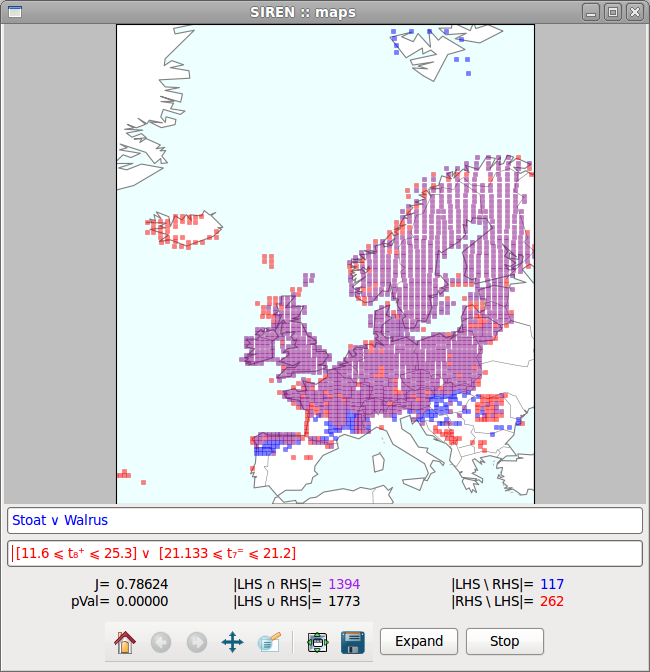
\includegraphics[width=.5\textwidth]{screenshots/siren_map.png}
%   \caption{Map panel, displaying a redescription on a map.}
%   \label{fig:map_panel}
% \end{figure}

% \begin{figure*}[t]
%   \centering
% %%FIG%%
% 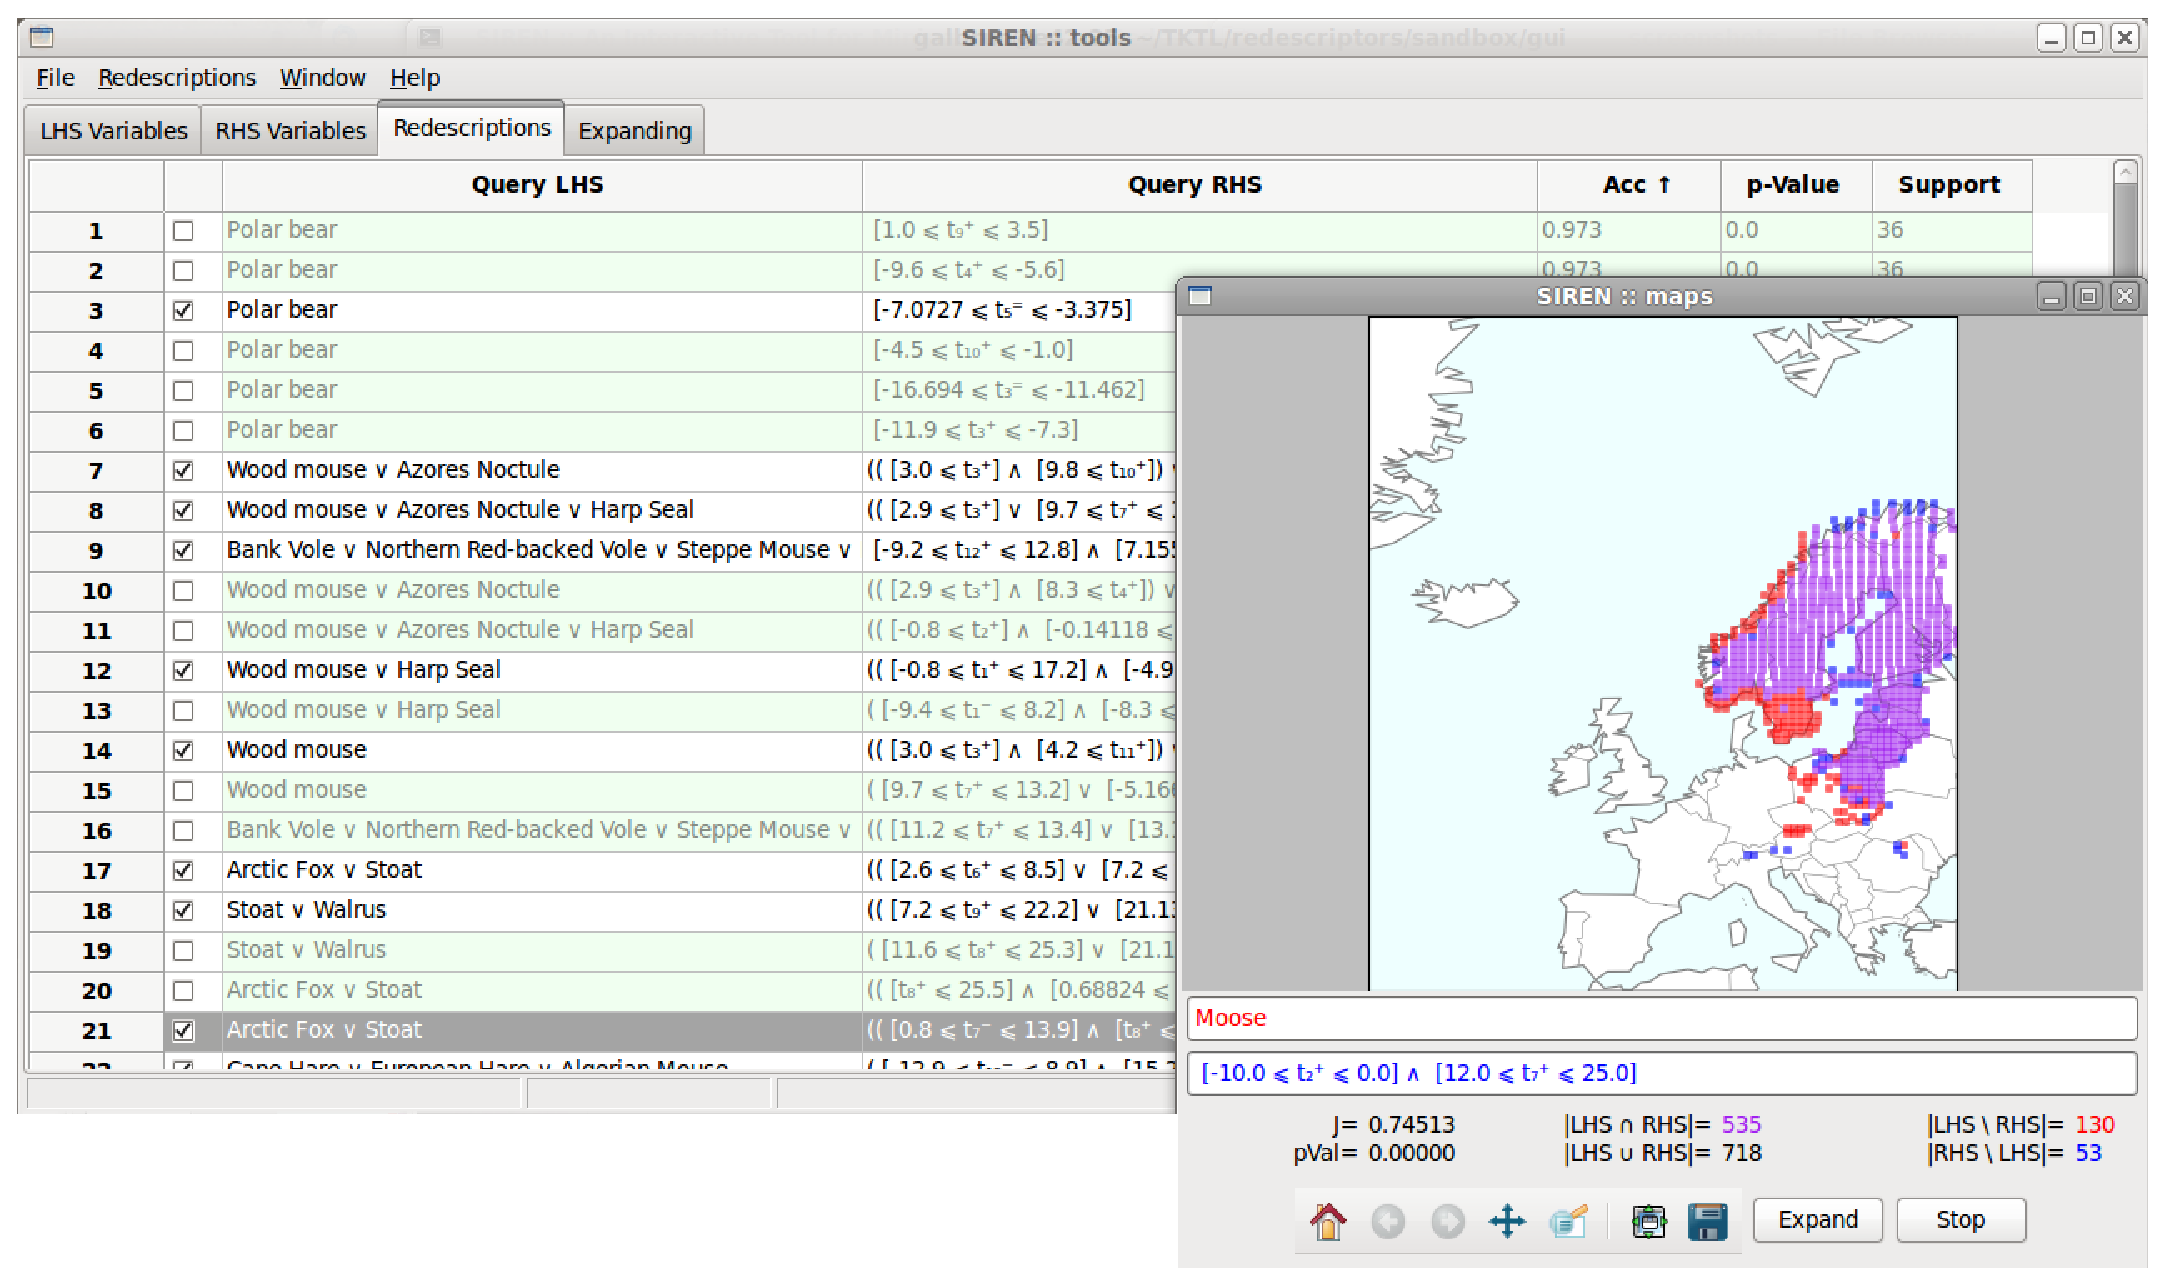
\includegraphics[width=\textwidth]{screenshots/both_panels_02}
%   \caption{The \Siren\ interactive mining and visualization tool. The panel in the background contains a list of redescriptions while the foreground panel displays the map of a selected redescription.  In this example, left hand side queries are over fauna while right hand side queries are over monthly bioclimatic conditions, that is, temperatures and precipitation.}
%   \label{fig:both_panels}
% \end{figure*}

% \begin{figure}
%   \centering
% 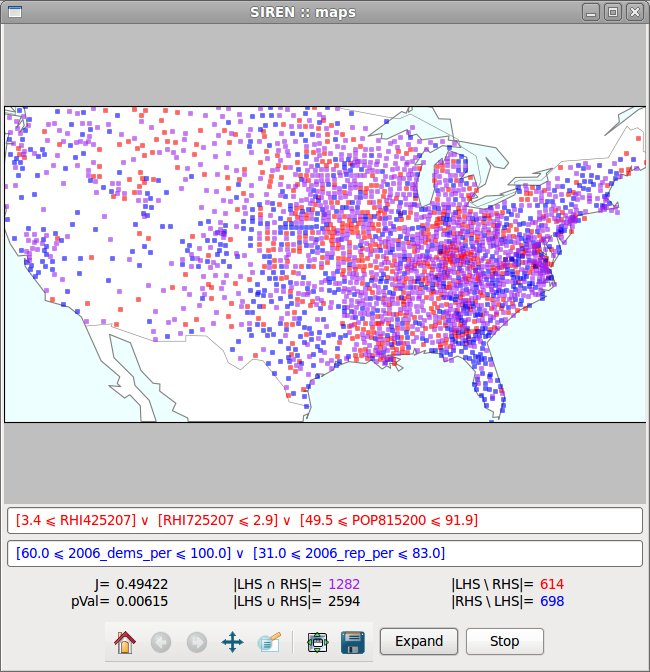
\includegraphics[width=.5\textwidth]{screenshots/siren_map_us_00.jpg}
%   \caption{Map panel, displaying a redescription on a map.}
%   \label{fig:map_panel}
% \end{figure}

% \begin{figure}
%   \centering
% 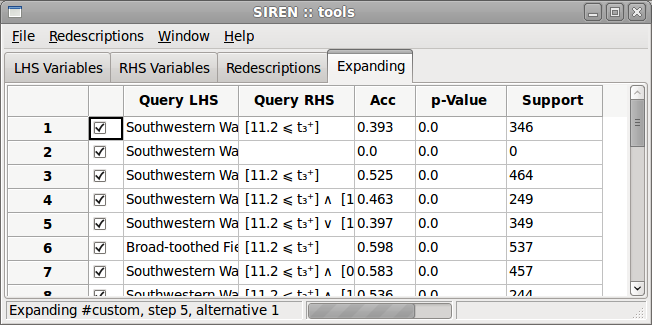
\includegraphics[width=0.5\textwidth]{screenshots/extending.png}
%   \caption{Tool panel. Intermediates results found during the extension of a redescription.}
%   \label{fig:extending}
% \end{figure}

% \begin{figure}
%   \centering
% %%FIG%%
% 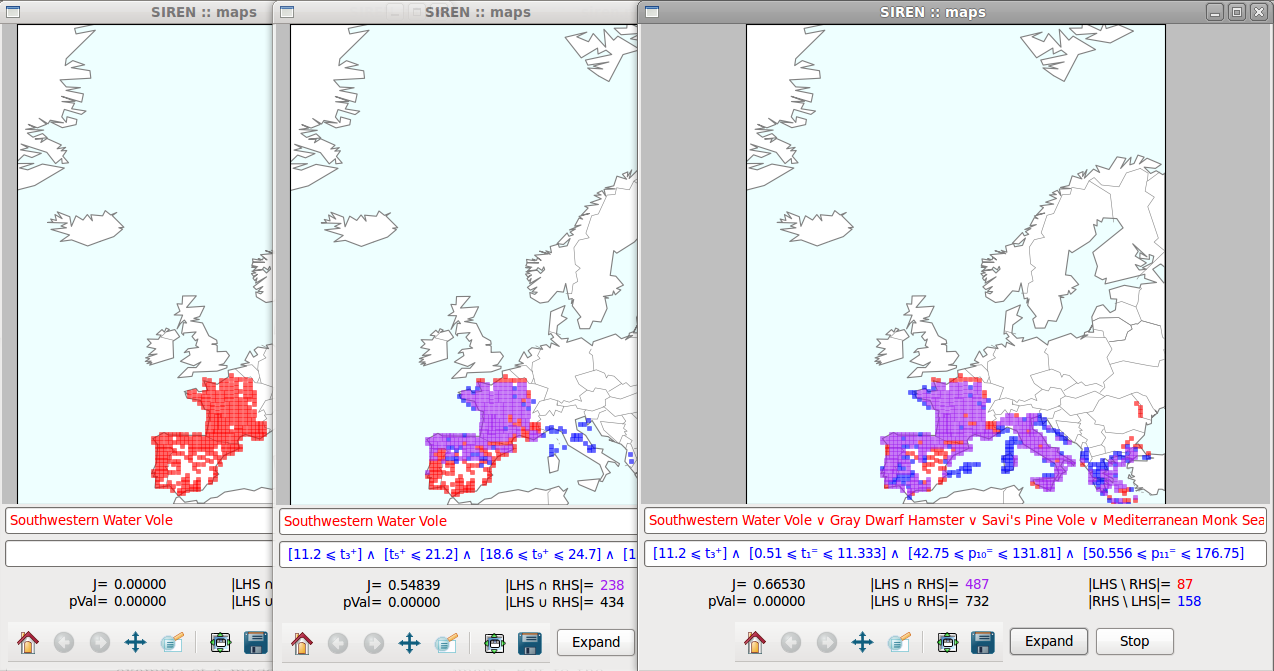
\includegraphics[width=0.7\textwidth]{screenshots/comparison}
%   \caption{Several map panels. Comparing intermediate extensions automatically generated for a chosen starting variable. Red, blue and purple represents areas where only the left hand side query holds, only the right hand side query holds and where both queries hold, respectively.}
%   \label{fig:comparison}
% \end{figure}


% \begin{figure}
%   \centering
% 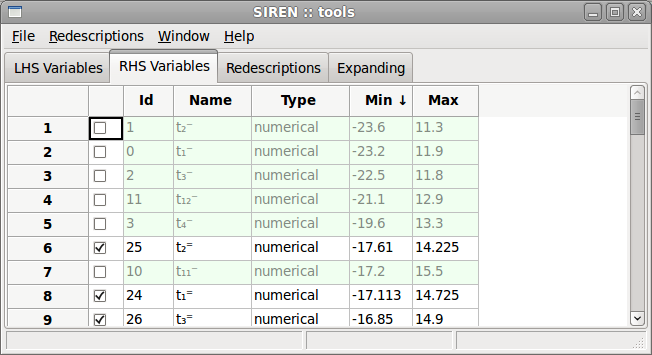
\includegraphics[width=.5\textwidth]{screenshots/variables_05.png}
%   \caption{Tool panel, uselecting variables.}
%   \label{fig:map_panel}
% \end{figure}

% \begin{figure}
%   \centering
% 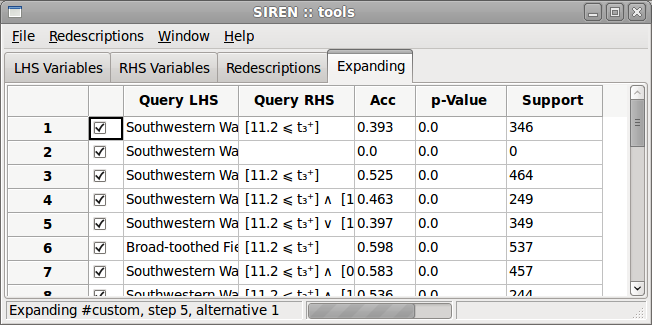
\includegraphics[width=0.5\textwidth]{screenshots/extending.png}
%   \caption{Tool panel, extending a redescription.}
%   \label{fig:extending}
% \end{figure}

% \begin{figure}
%   \centering
% 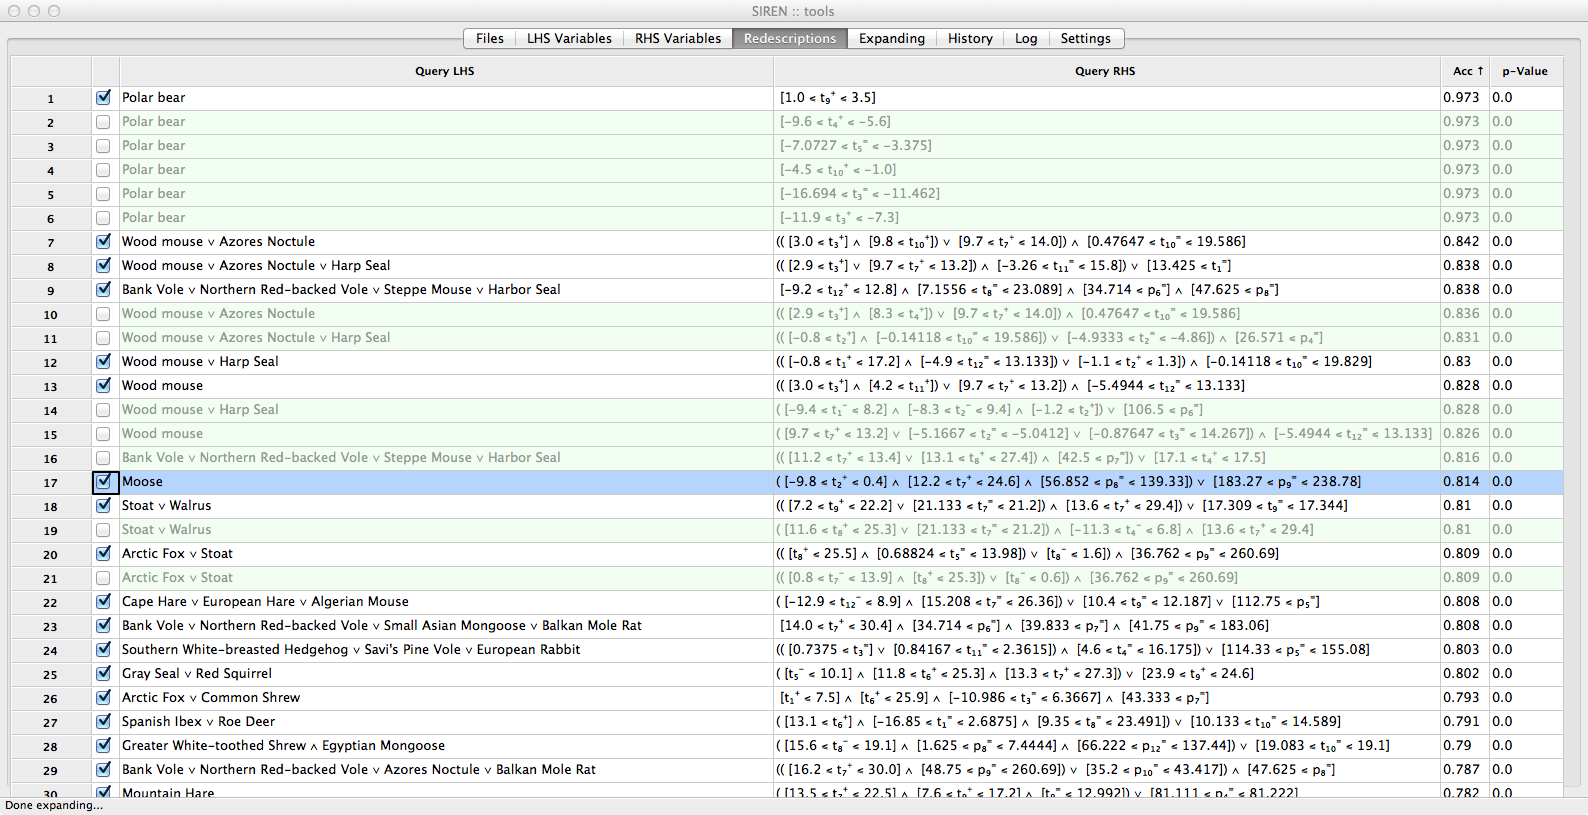
\includegraphics[width=.5\textwidth]{screenshots/redescriptions.png}
%   \caption{Tool panel, filtering redescriptions.}
%   \label{fig:filtering}
% \end{figure}
